
\section{Introduction to radio interferometric imaging}\label{intro2}
\begin{figure}[htp]
	% preliminary
	\sbox\twosubbox{%
		\resizebox{\dimexpr.9\textwidth-1em}{!}{%
			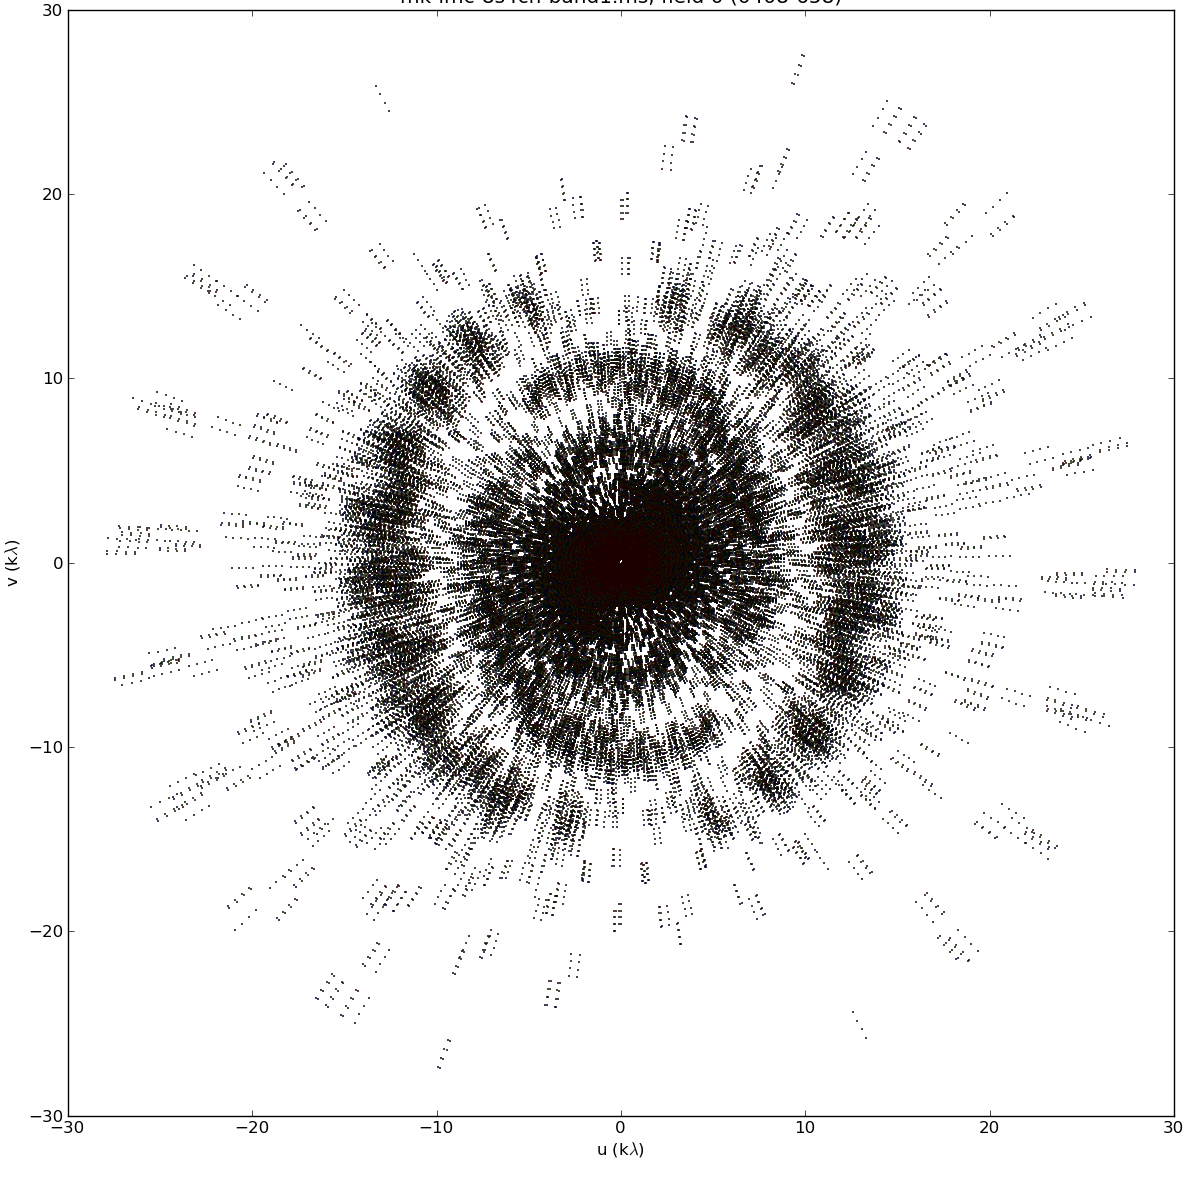
\includegraphics[height=3cm]{./chapters/01.intro/meerkat_uv2.png}%
			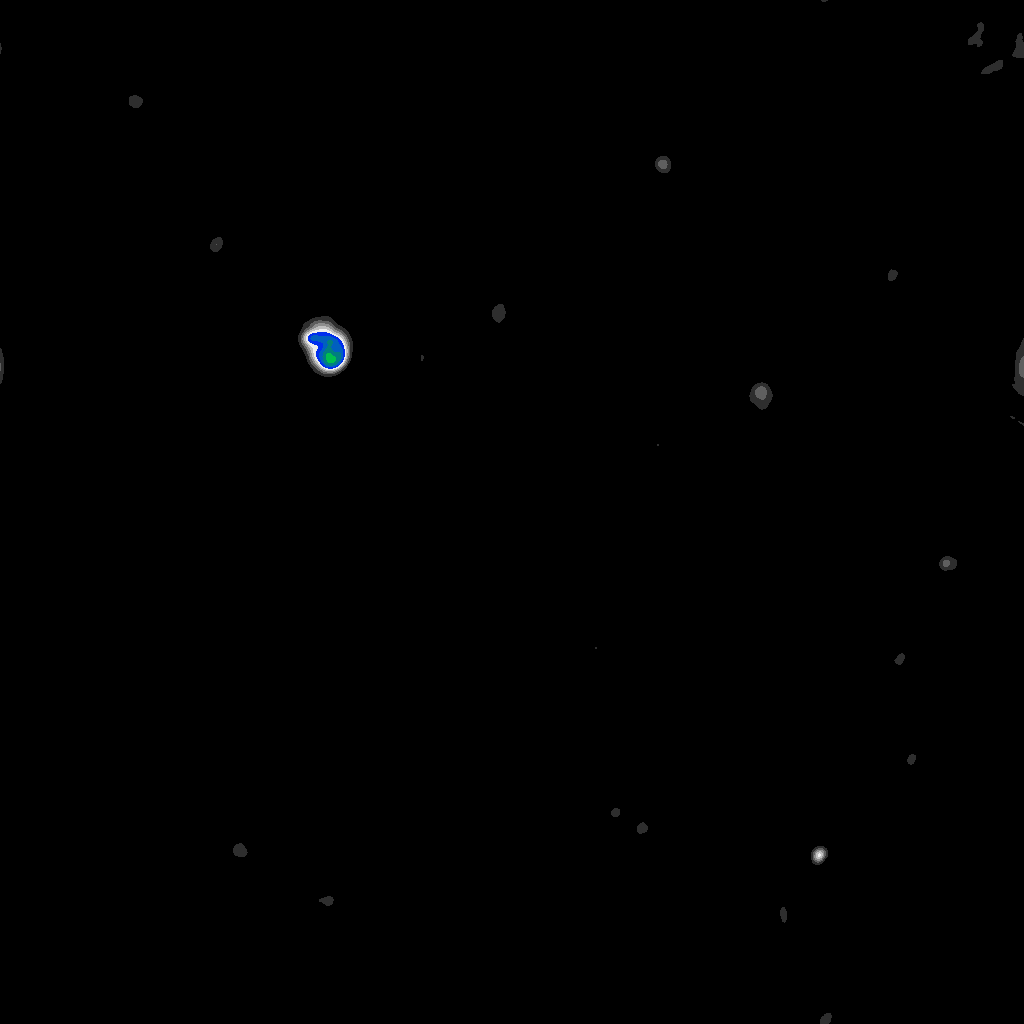
\includegraphics[height=3cm]{./chapters/01.intro/mk2/clean.png}%
		}%
	}
	\setlength{\twosubht}{\ht\twosubbox}
	
	% typeset
	\centering
	\subcaptionbox{Measurements in the Fourier space.\label{intro:inversefig:uvspace}}{%
		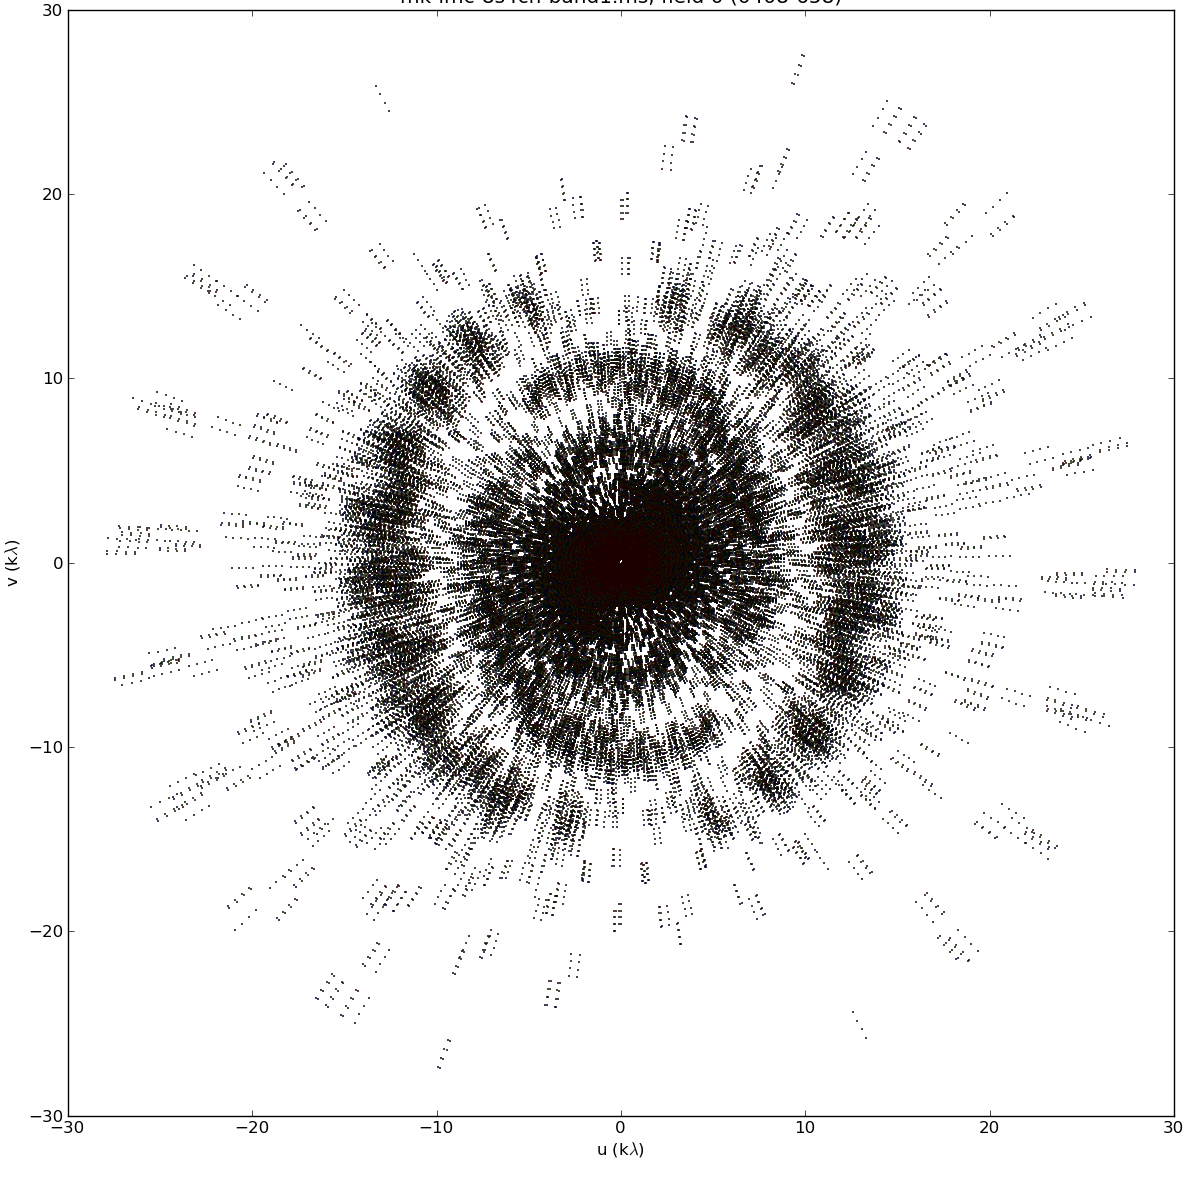
\includegraphics[height=\twosubht]{./chapters/01.intro/meerkat_uv2.png}%
	}\quad
	\subcaptionbox{Reconstructed image.\label{intro:inversefig:reconstruction}}{%
		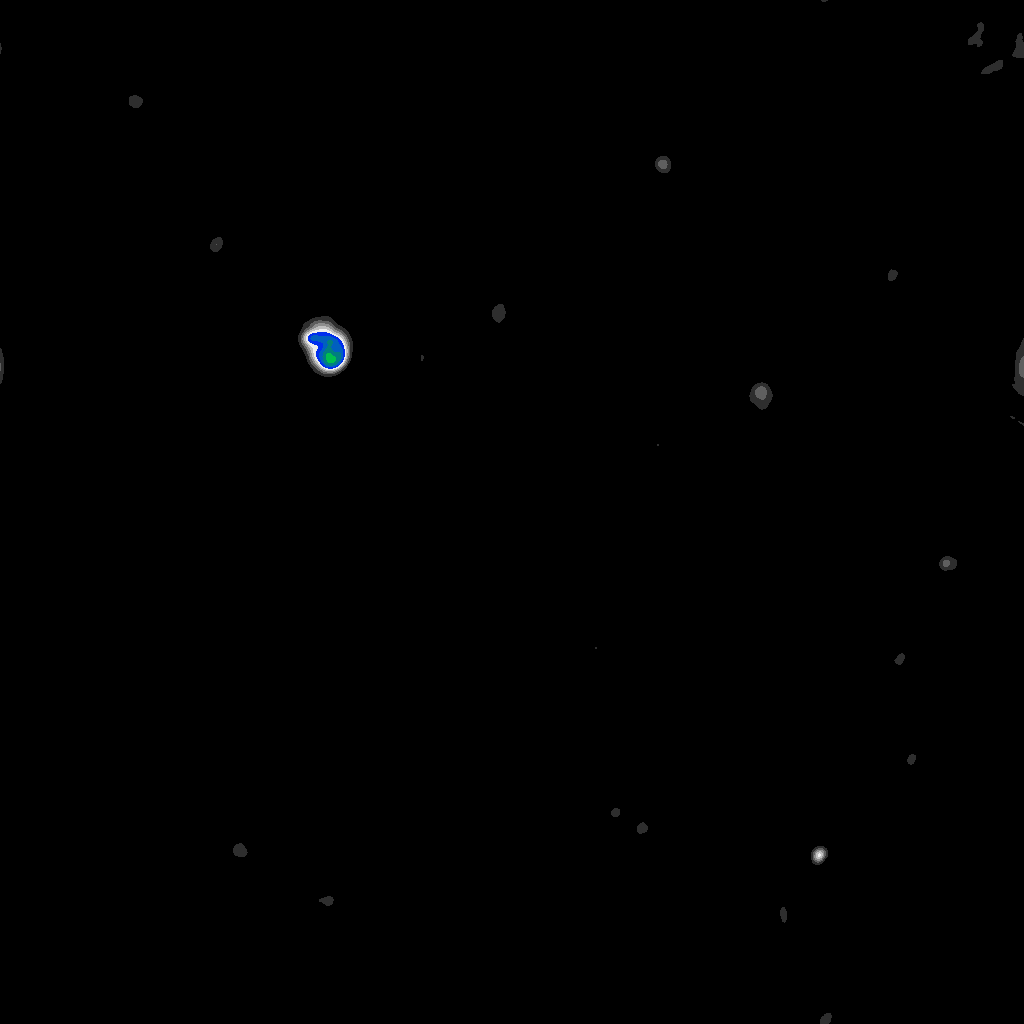
\includegraphics[height=\twosubht]{./chapters/01.intro/mk2/clean.png}%
	}
	\caption{Example of an image reconstruction for visibility measurements of the MeerKAT radio interferometer}\label{intro:inversefig}
\end{figure}

The figure \ref{intro:inversefig} gives an example of the radio interferometric imaging. We wish to reconstruct an image, shown in \ref{intro:inversefig:reconstruction} from the measurements of the interferometer \ref{intro:inversefig:uvspace}. The reconstructed image contains two object types: Point sources and extended emissions. Point sources, stars for example, are far-away emissions that are concentrated in a single pixel. Extended emissions like hydrogen clouds emit radio waves over a large area of the sky and span over several pixels in the reconstructed image.

The measurements of the radio interferometer are in the Fourier space. It does not measure how much emission was observed at a single pixel in the sky image, it measures the amplitude and phase of a Fourier component of the sky image. This means each dot in the figure \ref{intro:inversefig:uvspace} represents one Fourier measurement (amplitude and phase) of the observed image. The dots in the center, measurements with a low $uv$-value, measure the low-frequency components of the sky image. They contain the information about structures spanning over several pixels. Dots further away from the center measure the high-frequency components, they contain the information about the edges of the image and are responsible for a "sharp" image. In the radio astronomy literature, the measured Fourier components are called visibilities and for the sake of consistency, we will be calling the measured Fourier components visibilities in this work.

As we will see, we cannot retrieve the observed image by simply calculating the inverse Fourier transform. We require a reconstruction algorithm that finds the most likely observed image given the measurements. How close the most likely image is to the truly observed one depends on the reconstruction algorithm we choose. As it is often the case, how expensive an image reconstruction is in terms of runtime costs (Money spent on the necessary CPU's, time spent waiting for the results etc.) also depends on the reconstruction algorithm. We often face a trade-off between reconstruction quality and runtime costs. This work focuses on distributing the radio interferometric image reconstruction. We search for an effective way to use distributed computing hardware and test how scalable the reconstruction algorithm is with a real-world observation of the MeerKAT radio interferometer.

Introduction to how a radio interferometer works
What the fundamental problems are and how we can solve them in theory and what the implications are in practice
how we can 
This section gives a short introduction to interferometry and show the fundamental problems in the radio interferometric image reconstruction. In section \ref{intro2:ill-posed} we give an introduction how we can solve the radio interferometric image reconstruction in theory, and what the implications are in practice. Section \ref{intro2:rec} introduces how the common architecture for radio interferometric image reconstruction, and how the reconstruction algorithm is divided into sub-tasks in practice. 

\subsection{From electromagnetic waves over visibilities to images}
We give a short introduction into how the electromagnetic wave gets measured by the interferometer, turned into visibilities and finally processed into an image. Figure \ref{intro:system} shows a radio source and its electro-magnetic (e-m) wave arriving at the antennas of the interferometer. It then shows the three processes involved to arrive at an image: Correlation, calibration and image reconstruction.
	
\begin{figure}[h]
	\centering
	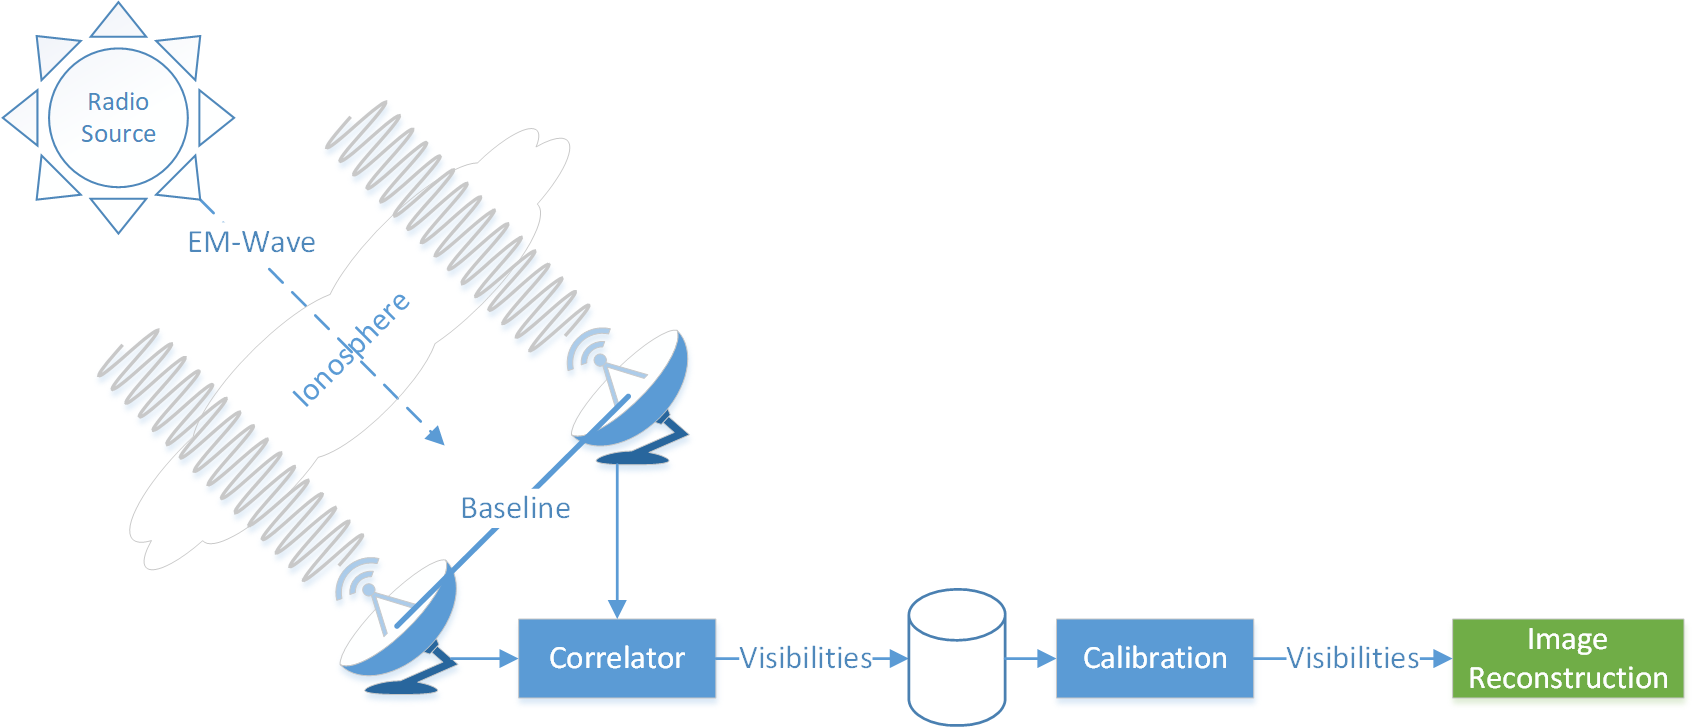
\includegraphics[width=0.80\linewidth]{./chapters/01.intro/system.png}
	\caption{Radio interferometer system}
	\label{intro:system}
\end{figure}

First, we have a source in the sky that is emitting e-m waves in the radio frequency. The waves travel to earth, through the earth's ionosphere and finally to our interferometer. Along its path, the e-m waves may get distorted from various sources. For example, it may receive a phase shift by the ionosphere.

Then, the e-m wave arrives at our interferometer. We call each antenna pair a baseline. Each baseline will end up measuring a single visibility. The figure \ref{intro:system} shows a single baseline of the interferometer. The distance between the antennas and their orientation to the e-m wave will determine where we sample the $uv$-plane. Short baselines measure the $uv$-plane close at the origin, while long baselines sample the $uv$-space further away from the origin. Remember that the samples away from the $uv$-origin contain the information about edges and other details of our image. With a longer baseline the interferometer measures more highly resolved details, regardless of the antenna dish-diameter\footnote{Remember that this is the reason why we build radio interferometers. We do not need impossibly large dish diameters for a high angular resolution. We just need large distances between smaller antennas}.

Not yet visibilities. This happens in the correlator
Correlator, amplitude and phase of the e-m wave at a frequency.
saved for further processing


Calibration. Effects from the ionosphere. Imperfections of the instrument, like varying antenna sensitivity.
Calibration is complex, and not part of the project

Image reconstruction generally happens after calibration. The focus of this project.
self-calibration

\subsubsection{The measurement equation}
As we discussed so far, the radio interferometer measures visibilities of the sky image, and we wish to find the observed image from the measurements. Put formally, we wish to invert the following system of linear equations \eqref{intro2:model:linear}, where $V$ is the visibility vector\footnote{We use the lower-case $v$ to denote the axis in the Fourier space $uvw$, and the upper-case letter to denote the visibility vector.}, $F$ is the Fourier transform matrix and $I$ is the pixel vector of the observed image.

\begin{equation}\label{intro2:model:linear}
V = F I
\end{equation}

We wish to find the observed image $I$, while we only know the visibility vector $V$ and the Fourier transform matrix $F$. This is what we call the measurement equation. In most context for this project, looking is an adequate view of the image reconstruction problem. We will show why we cannot find the observed image $I$ by simply calculating the inverse Fourier transform. However, when we need to efficiently apply the Fourier transform, we need to know $F$ in more detail. As we will see, radio interferometers have some difficulties hidden in the Fourier transform matrix, which are difficult to handle efficiently. First, let us abandon the vector notation of \eqref{intro2:model:linear}, and represent the measurement equation with integrals \eqref{intro2:model:smallfov}.

\begin{equation}\label{intro2:model:smallfov}
V(u, v) = \int\int I(l, m)  e^{2 \pi i [ul+vm]} \: dl \: dm
\end{equation}

This is essentially the same problem. The main difference is that we do not represent the Fourier transform as a matrix $F$, but as integrals $\int\int e^{2 \pi i [ul+vm]}$, where $u$, $v$ are the coordinates in Fourier space and $l$, $m$ are the angles away from the image center. A single pixel represents the intensity of the radio emission from the direction $l$, $m$. Note that the measurement equation \eqref{intro2:model:smallfov} shows the fact that the visibilities are measured in a continuous Fourier space. If the Fourier space would also be discrete, we could replace the integrals with sums.

However, the measurement equation \eqref{intro2:model:smallfov} is inaccurate in the sense that it ignores many effects that distort the signal. For example, it does not account for the distortion by the ionosphere, or the distortion introduced by real-world antennas. The measurement equation \eqref{intro2:model:smallfov} shown here does not represent the real world. But depending on the instrument and the observation, these distortions may be negligible, and the measurement equation \eqref{intro2:model:smallfov} is a good approximation. 

When there is a distortion source that cannot be ignored, it has to be modelled in the measurement equation. As such there is no unified measurement equation for all radio interferometric observations, let alone radio interferometers. The equation shown in \eqref{intro2:model:smallfov} can be seen as the basis that gets extended as necessary\cite{smirnov2011revisiting1, smirnov2011revisiting2, smirnov2011revisiting3, smirnov2011revisiting4}.

For example, the measurement equation \eqref{intro2:model:smallfov} is only accurate for small field of view observations, when $l$ and $m$ are both small angles. For wide field of view observations, we need to account for the fact that the visibilities have a third term $w$, and we arrive at the wide field of view measurement equation \eqref{intro2:model:widefov}.
 
\begin{equation}\label{intro2:model:widefov}
 V(u, v, w) = \int\int  \frac{I(l, m)}{c(l, m)}  e^{2 \pi i [ul+vm+ w(c(x, y) - 1)]} \: dl \: dm \:,  \quad c(l,m) = \sqrt{1 - l^2 - m ^2}
\end{equation}
 
The third $w$-term has two effects on the measurement equation. It introduces a phase shift in the Fourier transform $e^{2 \pi i [\ldots +w(c(l, m) - 1)]}$, and a normalization factor of the image $\frac{I(l, m)}{c(l, m)}$. Note that when the angles are small, i.e. $l^2 +m^2 \ll 1$ then the wide field of view measurement equation \eqref{intro2:model:widefov} reduces to our original \eqref{intro2:model:smallfov}. This is another way of saying that for small field of views, the measurement equation \eqref{intro2:model:smallfov} is a good approximation under the right conditions. 

In this project, we use the wide field of view measurement equation \eqref{intro2:model:widefov}. But as we mentioned in the beginning of this section, for most contexts, it is not important whether we ignore the $w$-term of the visibilities or not. It is important when we design an efficient implementations for applying the wide field of view Fourier transform, because the $w$-term keeps us from using the Fast Fourier Transform (FFT). In every other case, we can ignore this technicality. Because even more complicated measurement equation still have a linear relationship between visibilities and image \cite{smirnov2011revisiting1, smirnov2011revisiting2, smirnov2011revisiting3, smirnov2011revisiting4}. We can view the whole reconstruction problem as a system of linear equations \eqref{intro2:model:linear}, where the matrix $F$ takes care of how exactly the measurements and pixels relate in this case.

\subsection{The ill-posed image reconstruction problem}\label{intro2:ill-posed}
So far, we discussed how the interferometer measures in Fourier space, and we wish to find the observed image that matches the measurements. In other words, we wish to find a solution to a system of linear equation \eqref{intro2:ill-posed:linear}, where $V$ are the measurements, $x$ is the observed image and $F$ is the Fourier transform matrix. We also discussed that $F$ can be complicated in practice, but is still essentially a linear operator. Meaning we know how the inverse Fourier transform matrix $F^{-1}$, and the question arises: Why can't we solve the equations \eqref{intro2:ill-posed:linear} by calculating the inverse Fourier transform? Or, why does $x = F^{-1} V$ not lead to the observed image?

\begin{equation}\label{intro2:ill-posed:linear}
\underset{x}{solve}\quad V - Fx = 0
\end{equation}

The answer is, the equations \eqref{intro2:ill-posed:linear} do not have a unique solution, which makes the problem ill-posed. The problem is considered ill-posed when it has one of the following properties:
\begin{enumerate}
	\item No solution exists.
	\item There are solutions, but no unique solution exists.
	\item The solution behaviour does not change continuously with the initial condition (For example: a small change in the measurements lead to a very different reconstructed image).
\end{enumerate}
From linear algebra, we know that an under-determined system of linear equations, i.e. when \eqref{intro2:ill-posed:linear} has more pixels than visibility measurements, then the problem is under-determined and there may be a potentially infinite number of solutions to the system. Under-determined systems arise in many similar fields, as for example in X-Ray imaging of the sun\cite{felix2017compressed}. However, radio interferometers measure a large number of visibilities. We generally have more visibilities than pixels. This means the image reconstruction problem \eqref{intro2:ill-posed:linear} for radio interferometers is actually over-determined.

From linear algebra, we know that an over-determined system either has one or zero solutions. At first glance it may be counter-intuitive why there are many possible solutions to \eqref{intro2:ill-posed:linear} for radio interferometers. The reason why lies in two properties of the measurements: They are noisy and incomplete.

The radio interferometer measures noisy visibilities, meaning each amplitude and phase of a measurement is influenced by an unknown noise factor. Finding a reconstructed image is the same as finding the de-noised versions of the visibility measurements. This alone would make the problem ill-posed, but the visibilities actually have a second property that makes them ill-posed: incompleteness.

When we look back at figure \ref{intro:inversefig:uvspace}, it is clear to see that the interferometer does not sample the visibilities in a uniform way. There are regions with a high sample density. The density decreases when we move further away from the center. The higher frequency visibilities get fewer and fewer samples. This means we are missing data for crucial measurements for the reconstruction.

Also note that the question whether the measurements are incomplete essentially comes down to the image resolution of the reconstruction: Since we are missing high-frequency measurements and we can choose the resolution of the image, we can also reduce the resolution of the reconstructed image until the missing frequencies become negligible. However, if we can solve the ill-posed inverse problem, we can reconstruct an image at a higher resolution from the same measurements. The question is how do we solve the ill-posed inverse problem?

\subsubsection{Adding a regularization} \label{intro:linear:regularization}
For ill-posed inverse problems, there are two viewpoints for the same idea. From the viewpoint of optimization, we can solve the ill-posed image reconstruction problem \eqref{intro:linear:linear} by adding a regularization. The regularization creates a system of linear equations with a unique solution. From the viewpoint of Bayesian Statistics, we include prior knowledge about the image, and therefore search the most likely image given the measurements. For this project, both terms describe the same idea and we use regularization and prior interchangeably. We know that the reconstructed image from radio interferometers contain a mixture of stars (point sources located in a single pixel) and extended emissions like hydrogen clouds. By adding this prior knowledge to the reconstruction problem, we can find the most likely image given the measurements. As we will see, under the right prior, we can create a reconstruction algorithm that is almost guaranteed to find the truly observed image in theory.

There are different ways to include regularization in the reconstruction problem. In this project, we use the following method: We cast the image reconstruction problem into an optimization objective consisting of a data fidelity term and a regularization term. A reconstruction algorithm therefore consists of an optimization objective, a prior function and an optimization algorithm.

\begin{equation}\label{intro:linear:compressed}
\underset{x}{minimize} \: \left \| V - Fx \right \|_2^2 + \lambda P(x)
\end{equation}

The objective \eqref{intro:linear:compressed} has a data term $\left \| V - Fx \right \|_2^2$, which forces the most likely image to be as close to the measurements as possible, and the regularization term $P(x)$, which penalizes unlikely images according to our prior function. The parameter $\lambda$ represents how much we penalize unlikely images and by extend, much noise we expect in the reconstruction. The parameter $\lambda$ is either left to the user to define, can be estimated from the data \cite{miller1970least}. 

The prior function $P()$ represents our prior knowledge about the image. It assigns a high penalty for unlikely images. In in radio interferometric image reconstructions tend to use similar prior functions as for image de-noising applications. Such as: Total Variation ($\left \| \triangledown x \right \|_1$) \cite{wiaux2009compressed}, L2 ($\left \|x \right \|_2$) \cite{ferrari2014distributed} or the L1 norm in a wavelet space ($\left \|\Psi x \right \|_1$) \cite{girard2015sparse}.

Finally, an optimization algorithm is necessary which can optimize the objective function \eqref{intro:linear:compressed} with the chosen prior function $P()$. Typical choices for optimization algorithms in image reconstructions are Interior Point Methods like Simplex, Matching Pursuit \cite{hogbom1974aperture} and ADMM\cite{carrillo2014purify}. 

A reconstruction algorithm for radio astronomy consists of an optimization objective, a prior function and an optimization algorithm. It is a three dimensional design space. Not every prior is suitable for every optimization algorithm. The choice of optimization objective influences both what prior and what optimization algorithm we can use. Although there are a different choices for the optimization objective, we limit ourselves to the objective \eqref{intro:linear:compressed} and explore how we can distribute the reconstruction problem.

The last question that remains is, how close are the most likely image, under a given prior, to the truly observed one? Remember that the Nyquist-Shannon sampling theorem states that our uniform sampling frequency needs to be larger than twice the highest frequency in a band-limited signal\footnote{For example: if we want to record human voices with the highest frequency of 20 kHz, Nyquist-Shannon states our uniform sampling frequency has to be larger than 40 kHz to guarantee exact reconstruction}, and then the theorem guarantees exact reconstruction. For radio astronomy, we do not have uniformly sampled visibilities, and although we have a large number of samples, we are missing crucial parts of the Fourier space. Luckily, there is another sampling theorem that, under certain assumptions, guarantees exact reconstruction for the case of radio interferometers. Namely, the theory of compressed sensing.

\subsubsection{Compressive sampling of the sky}
For the sake of demonstration, let us assume the radio interferometer observes a patch of sky containing ten stars. It measures an incomplete set of random Fourier components of the ten stars, and we would like to reconstruct an image of size $256^2$ pixels. The emissions from stars are concentrated into a single pixel. For compressive sampling, we need to know an space in which our reconstructed image is sparse, and we need to take measurements in a different, incoherent space.

Our reconstructed image contains only zero pixels except at the ten locations of the stars, meaning the image space for this patch of the sky is already sparse. In this case, we do not need any additional sparse space like wavelets. We can reconstruct directly in the sparse image space, and we have the first requirement met for compressive sampling. 

The next requirement is that the measurement and reconstruction space (which is the image in this example), are as incoherent as possible. 

Yes, incoherence.
\begin{equation}\label{intro:linear:compressed2}
\underset{x}{minimize} \: \left \| V - Fx \right \|_2^2 + \lambda \left \| x \right \|_1
\end{equation}


Intuitively, the number of samples depend on the information content, not on the bandwidth. thi


At what point are we guaranteed? The matrix $A$ needs to fullfil the Restricted Isometry Porperty (RIP) \cite{candes2006robust,donoho2006compressed}.
Approximately orthonormal on sparse signals. (If we randomly choose ten columns of $F$, how much do they correlate. We want as little correlation as possible.)
Calculate the RIP is NP-hard\cite{tillmann2013computational}. Approximations are also difficult to compute\cite{natarajan2014computational}.
So we can only talk about how likely a given matrix fullfils the RIP. Matrix where each element is sampled from a random Gaussian distributîon has the highest change.

Random samples in the Fourier space also have a high chance to fulfill the RIP \cite{haviv2017restricted}.

Not possible for Radio interferometers, because they sample in the Fourier space. Not random.

There are also extended emissions, clouds etc. Resulting in a lot of non-zero pixels. There may be better sparse spaces for radio astronomy.

But also RIP may be too strict. Exact reconstruction can also work under less strict conditions\cite{candes2011probabilistic} active field of research.

\subsubsection{Reconstruction guarantees in the real world}

What does this all mean for image reconstruction?
For us, we design reconstruction algorithms and cannot influence the matrix $F$. We do not know if it actually 

The theory of compressed sensing gives us a framework. There is a data modelling task, and a task for finding efficient algorithms.

So there is a data modelling task in finding a good sparse prior.
We also do not know the proper sparse space in which radio interferometric images. We know several spaces, Curvelets \cite{starck2003astronomical} Starlets \cite{starck2015starlet}, Daubechies wavelets \cite{carrillo2012sparsity}. As of the time of writing, it is currently unknown which leads to the best reconstruction.
We can also learn dictionaries.

The task for efficient algorithms is finding the best way to optimize the objective with a given prior on real hardware. Fast convergence. Also difficult, because in practice the choice of prior can also influence convergence.


Compressed sensing based reconstruction algorithm. In radio astronomy.








\subsection{Introduction into optimization/RI reconstruction algorithms}\label{intro2:rec}

\subsubsection{The Major/Minor cycle}\label{intro2:opt:cycle}

\subsubsection{Image reconstruction as deconvolution}
